%%
%% This is file `sample-sigconf.tex',
%% generated with the docstrip utility.
%%
%% The original source files were:
%%
%% samples.dtx  (with options: `sigconf')
%% 
%% IMPORTANT NOTICE:
%% 
%% For the copyright see the source file.
%% 
%% Any modified versions of this file must be renamed
%% with new filenames distinct from sample-sigconf.tex.
%% 
%% For distribution of the original source see the terms
%% for copying and modification in the file samples.dtx.
%% 
%% This generated file may be distributed as long as the
%% original source files, as listed above, are part of the
%% same distribution. (The sources need not necessarily be
%% in the same archive or directory.)
%%
%% The first command in your LaTeX source must be the \documentclass command.
\documentclass[sigconf]{acmart}

%%
%% \BibTeX command to typeset BibTeX logo in the docs
\AtBeginDocument{%
  \providecommand\BibTeX{{%
    \normalfont B\kern-0.5em{\scshape i\kern-0.25em b}\kern-0.8em\TeX}}}

%% Rights management information.  This information is sent to you
%% when you complete the rights form.  These commands have SAMPLE
%% values in them; it is your responsibility as an author to replace
%% the commands and values with those provided to you when you
%% complete the rights form.
%\setcopyright{acmcopyright}
%\copyrightyear{2018}
%\acmYear{2018}
%\acmDOI{10.1145/1122445.1122456}

%% These commands are for a PROCEEDINGS abstract or paper.
%\acmConference[Woodstock '18]{Woodstock '18: ACM Symposium on Neural
%  Gaze Detection}{June 03--05, 2018}{Woodstock, NY}
%\acmBooktitle{Woodstock '18: ACM Symposium on Neural Gaze Detection,
%  June 03--05, 2018, Woodstock, NY}
%\acmPrice{15.00}
%\acmISBN{978-1-4503-XXXX-X/18/06}


%%
%% Submission ID.
%% Use this when submitting an article to a sponsored event. You'll
%% receive a unique submission ID from the organizers
%% of the event, and this ID should be used as the parameter to this command.
%%\acmSubmissionID{123-A56-BU3}

%%
%% The majority of ACM publications use numbered citations and
%% references.  The command \citestyle{authoryear} switches to the
%% "author year" style.
%%
%% If you are preparing content for an event
%% sponsored by ACM SIGGRAPH, you must use the "author year" style of
%% citations and references.
%% Uncommenting
%% the next command will enable that style.
%%\citestyle{acmauthoryear}

%\usepackage[table,xcdraw]{xcolor}
\usepackage{colortbl}
\usepackage[ruled,vlined]{algorithm2e}
\usepackage{graphicx,color}
\usepackage{booktabs}
\usepackage{listings}

\lstdefinelanguage[RISC-V]{Assembler}
{
  alsoletter={.}, % allow dots in keywords
  alsodigit={0x}, % hex numbers are numbers too!
  morekeywords=[1]{ % instructions
    lb, lh, lw, lbu, lhu,
    sb, sh, sw,
    sll, slli, srl, srli, sra, srai,
    add, addi, sub, lui, auipc,
    xor, xori, or, ori, and, andi,
    slt, slti, sltu, sltiu,
    beq, bne, blt, bge, bltu, bgeu,
    j, jr, jal, jalr, ret,
    scall, break, nop, li, ffred, ffwidth, clmul
  },
  morekeywords=[2]{ % sections of our code and other directives
    .align, .ascii, .asciiz, .byte, .data, .double, .extern,
    .float, .globl, .half, .kdata, .ktext, .set, .space, .text, .word
  },
  morekeywords=[3]{ % registers
    zero, ra, sp, gp, tp, s0, fp,
    t0, t1, t2, t3, t4, t5, t6,
    s1, s2, s3, s4, s5, s6, s7, s8, s9, s10, s11,
    a0, a1, a2, a3, a4, a5, a6, a7,
    ft0, ft1, ft2, ft3, ft4, ft5, ft6, ft7,
    fs0, fs1, fs2, fs3, fs4, fs5, fs6, fs7, fs8, fs9, fs10, fs11,
    fa0, fa1, fa2, fa3, fa4, fa5, fa6, fa7
  },
  morecomment=[l]{;},   % mark ; as line comment start
  morecomment=[l]{\#},  % as well as # (even though it is unconventional)
  morestring=[b]",      % mark " as string start/end
  morestring=[b]'       % also mark ' as string start/end
}

% define some basic colors
\definecolor{mauve}{rgb}{0.58,0,0.82}

\lstset{
  % listings sonderzeichen (for german weirdness)
  literate={ö}{{\"o}}1
           {ä}{{\"a}}1
           {ü}{{\"u}}1,
  breaklines=true,                              % break long lines
  commentstyle=\itshape\color{green!50!black},  % comments are green
  keywordstyle=[1]\color{blue!80!black},        % instructions are blue
  keywordstyle=[2]\color{orange!80!black},      % sections/other directives are orange
  keywordstyle=[3]\color{red!50!black},         % registers are red
  stringstyle=\color{mauve},                    % strings are from the telekom
  identifierstyle=\color{teal},                 % user declared addresses are teal
  language=[RISC-V]Assembler,                   % all code is RISC-V
  tabsize=4,                                    % indent tabs with 4 spaces
  showstringspaces=false                        % do not replace spaces with weird underlines
}

\hyphenation{crypto-gra-phy cla-ssic algo-rithms algo-rithm proce-ssing accele-ra-tion ins-truction bet-ween appli-cations commu-nication ope-rations proce-ssor}

%%
%% end of the preamble, start of the body of the document source.
\begin{document}

%%
%% The "title" command has an optional parameter,
%% allowing the author to define a "short title" to be used in page headers.
\title{RISC-V ISA Extension for Galois Field arithmetic}

%%
%% The "author" command and its associated commands are used to define
%% the authors and their affiliations.
%% Of note is the shared affiliation of the first two authors, and the
%% "authornote" and "authornotemark" commands
%% used to denote shared contribution to the research.
\author{Yao-Ming Kuo}
\orcid{0001-9752-6073}
\author{Francisco García-Herrero}
\orcid{0001-6719-9681}
\author{Juan Antonio Maestro}
\orcid{0001-7133-9026}
\email{{ykuo1 ,fgarciahe, jmaestro}@nebrija.es}
\affiliation{%
  \institution{ARIES Research Center, Universidad Antonio de Nebrija}
  \streetaddress{C/ Pirineos, 55}
  \state{Madrid}
  \country{Spain}
  \postcode{28040}
}

%%
%% By default, the full list of authors will be used in the page
%% headers. Often, this list is too long, and will overlap
%% other information printed in the page headers. This command allows
%% the author to define a more concise list
%% of authors' names for this purpose.
%\renewcommand{\shortauthors}{Trovato and Tobin, et al.}

%%
%% The abstract is a short summary of the work to be presented in the
%% article.
\begin{abstract}
  With the rise of Edge Computing and the advancement of cryptography and error correction codes, 
  portable device processors must handle a wide range of algorithms. A tradeoff between speed and area must be found to speed up 
  the execution time of a general-purpose processor. As $GF(2^m)$ arithmetic is the basis of many algorithms, 
  an RISC-V instruction set extension is proposed in this work. The hardware is implemented, and the 
  results are validated using SweRVolf SoC (SweRV EL2 1.3) on a Nexys A7 FPGA. Performance in some algorithms has been improved 
  at the expense of a slight increase in logic utilization.
\end{abstract}

%%
%% The code below is generated by the tool at http://dl.acm.org/ccs.cfm.
%% Please copy and paste the code instead of the example below.
%%

\begin{CCSXML}
  <ccs2012>
     <concept>
         <concept_id>10010520.10010521.10010522.10010523</concept_id>
         <concept_desc>Computer systems organization~Reduced instruction set computing</concept_desc>
         <concept_significance>500</concept_significance>
         </concept>
     <concept>
         <concept_id>10002978.10002979</concept_id>
         <concept_desc>Security and privacy~Cryptography</concept_desc>
         <concept_significance>300</concept_significance>
         </concept>
     <concept>
         <concept_id>10002978.10003001.10003599</concept_id>
         <concept_desc>Security and privacy~Hardware security implementation</concept_desc>
         <concept_significance>300</concept_significance>
         </concept>
     <concept>
         <concept_id>10010583.10010588</concept_id>
         <concept_desc>Hardware~Communication hardware, interfaces and storage</concept_desc>
         <concept_significance>300</concept_significance>
         </concept>
   </ccs2012>
\end{CCSXML}
  
\ccsdesc[500]{Computer systems organization~Reduced instruction set computing}
\ccsdesc[300]{Security and privacy~Cryptography}
\ccsdesc[300]{Security and privacy~Hardware security implementation}
\ccsdesc[300]{Hardware~Communication hardware, interfaces and storage}

%%
%% Keywords. The author(s) should pick words that accurately describe
%% the work being presented. Separate the keywords with commas.
\keywords{RISC-V, ISA, Galois Field Arithmetic}

%% A "teaser" image appears between the author and affiliation
%% information and the body of the document, and typically spans the
%% page.
%\begin{teaserfigure}
%  \includegraphics[width=\textwidth]{sampleteaser}
%  \caption{Seattle Mariners at Spring Training, 2010.}
%  \Description{Enjoying the baseball game from the third-base
%  seats. Ichiro Suzuki preparing to bat.}
%  \label{fig:teaser}
%\end{teaserfigure}

%%
%% This command processes the author and affiliation and title
%% information and builds the first part of the formatted document.
\maketitle

\section{Introduction}
In recent decades, with the rise of small portable devices for applications such as the Internet of Things \cite{5579543}
and CubeSats \cite{heidt2000cubesat}, as well as the concepts of Edge Computing \cite{7488250}, Industry 4.0 \cite{lasi2014industry}, 
and Big Data, processors must be more efficient to execute specific operations and be able to attend the tasks with lower latency.


The first step is to identify the algorithms that are most used in a specific application. 
Once identified, a solution must be found to accelerate the processor, reducing the number of instructions, 
clock cycles, and power consumption. We have identified that cryptography and communication 
(Error Correction Codes) are present in almost any portable device today. 
Because of this, the acceleration of finite field arithmetic $GF(2^m)$ proceeds to have a significant role. 
It is generally used to encode and decode in a communication channel and detect errors in the transmitted data 
(BCH, Reed-Solomon codes). It is also used in asymmetric cryptography, such as Elliptical Curve Cryptography, 
which is extensively used in the authentication process to exchange private keys or symmetric cryptography 
inside a secure communication channel as Advanced Encryption Standard (AES).


Furthermore, quantum-resistant cryptography algorithms (PQC) \cite{8791343} have been developed in recent years 
with the rise of quantum computing research. Some of the survivors of the third round of the NIST's PQC competition \cite{moody2016post} 
use $GF(2^m)$ arithmetic (Classic McEliece \cite{bernstein2017classic}, Rainbow \cite{10.1007/11496137_12}, HQC \cite{melchor2018hamming}, and GeMSS \cite{casanova2017gemss}). 
These algorithms require high computing power to generate the keys and encrypt/decrypt the data, 
becoming the main bottleneck in processing for small devices.


Traditionally, there are three ways to optimize a processor. The first solution is adding coprocessors 
to the system to perform those specific operations. The second is expanding the base instructions 
of architecture. Moreover, the third solution is to make a hybrid system between the first and 
the second solution, adding coprocessors and specific instructions depending on the case. 
This work focuses on expanding RISC-V base instructions. This paper aims to propose a flexible instruction set 
capable of accelerating any algorithm based on finite field arithmetic $GF(2^m)$, thus improving processor performance.


The rest of the paper is organized as follows. Section 2 describes the mathematical basis of $GF(2^m)$, previous works, 
and contributions of this work. Section 3 presents the instruction set extension. Section 4 shows the simulations and 
experimental results in a RISC-V SoC (SweRVolf). Finally, section 5 presents the conclusion of this work.




\section{Background}
This section is divided into three subsections. The first describes the fundamentals of finite field arithmetic. 
Then, the second subsection details the previous related works. And finally, in the last subsection, 
the contributions of this work are listed.

\subsection{Finite field arithmetic}

In this subsection, a quick review of the concepts related to Galois Field operators is made (for more details, refer to \cite{deschamps2009hardware}), 
focused on GF($2^m$). This field is an extension of GF(2), where the elements that make it up are zero and one. 
All finite fields have a unit element ($\alpha^0$), a zero element ($\alpha^{-\infty}$), a primitive element ($\alpha$), and at least one irreducible polynomial 
$p(x) = x^m + p_{m-1}x^{m-1} + ... + p_{1}x + p_{0}$. The primitive element $\alpha$ is the root of the irreducible polynomial and 
generates all the GF($2^m$) nonzero elements.


There are two ways to represent the elements in GF($2^m$): exponential and polynomial. 
In the exponential representation, the parts are defined as powers of $\alpha$, i.e.
\begin{equation}
 GF (2^m) = \{ 0, \alpha^0, \alpha^1, \alpha^2, ..., \alpha^{2m-2}  \}
 \label{eq:1}
\end{equation}
While the polynomial representation has the following form:
\begin{equation}
\begin{split}
 P(\alpha) = a_{m-1}\alpha^{m-1} + ... + a_{1}\alpha + a_{0};\\ 
 a_{i} \in GF(2), 0 \leq i \leq m-1
 \end{split}
 \label{eq:2}
\end{equation}


Polynomial representation is beneficial for doing arithmetic operations. %\cite{Jain1998}. 
The definitions of addition and multiplication of finite fields are given below.


\subsubsection{GF Addition}
Let's consider two elements of $a(x)$ and $a(x)$ (Eq. \ref{eq:3}), both belonging to the field $GF(2^m)$.
\begin{equation}
\begin{split}
 a(x) = a_{m-1}x^{m-1} + ... + a_{1}x + a_{0}\\
 b(x) = b_{m-1}x^{m-1} + ... + b_{1}x + b_{0}\\
 a_{i} \wedge b_{i} \in GF(2), 0 \leq i \leq m-1
 \end{split}
 \label{eq:3}
\end{equation}
The sum $s(x)$ (Eq. \ref{eq:4}) is directly the XOR operation of each of its coefficients. The result belongs to the same field.

\begin{equation}
 s(x) = (a_{m-1} \oplus b_{m-1})x^{m-1} + ... + (a_{0} \oplus b_{0})
 \label{eq:4}
\end{equation}


\subsubsection{GF Multiplication} \label{section:gf_mult}

There are different ways to multiply two polynomials in $GF(2^m)$. This paper focuses on two-step multiplication. As its name implies, 
this method separates multiplication into two steps: carry-less multiplication and polynomial reduction.


The first step is carry-less multiplication. The product $d(x)$ of the polynomials $a(x)$ and $b(x)$, is a polynomial of degree $2m-2$. 
This operation can be represented in matrix form as:

\begin{equation}
    \begin{pmatrix}
    d_{0} \\
    d_{1} \\
    \vdots \\
    d_{m-1} \\
    d_{m} \\
    d_{m+1} \\
    \vdots \\
    d_{2m-2} \\
    \end{pmatrix}
    =
    \begin{pmatrix}
        a_{0} & 0 & 0 & \cdots & 0 & 0 \\
        a_{1} & a_{0} & 0 & \cdots & 0 & 0 \\
        \vdots & \vdots & \vdots & \ddots & \vdots & \vdots \\
        a_{m-1} & a_{m-2} & a_{m-3} & \cdots & a_{1} & a_{0} \\
        0 & a_{m-1} & a_{m-2} & \cdots & a_{2} & a_{1} \\
        0 & 0 & a_{m-1} & \cdots & a_{3} & a_{2} \\
        \vdots & \vdots & \vdots & \ddots & \vdots & \vdots \\
        0 & 0 & 0 & \cdots & 0 & a_{m-1} 
    \end{pmatrix}
    \begin{pmatrix}
        b_{0} \\
        b_{1} \\
        b_{2} \\
        \vdots \\
        b_{m-2} \\
        b_{m-1} 
    \end{pmatrix}
\end{equation}

After the carry-less multiplication, the next step is the polynomial reduction based on an 
irreducible polynomial $f(x)$. In modular reduction $c(x) = d(x) mod f(x)$, the degree of $d(x)$ is 
reduced by the degree of the irreducible polynomial $f(x)$, resulting in a degree less than $m – 1$.
The matrix form of the polynomial reduction is showed in Equation \ref{eq:red}.


\begin{equation}\label{eq:red}
    \begin{pmatrix}
        c_{0} \\
        c_{1} \\
        \vdots \\
        c_{m-1} \\
    \end{pmatrix}
    =
    \begin{pmatrix}
        1 & 0 & \cdots & 0 & r_{0,0} & \cdots & r_{0,m-2} \\
        0 & 1 & \cdots & 0 & r_{1,0} & \cdots & r_{1,m-2} \\
        \vdots & \vdots & \ddots & \vdots & \vdots & \ddots & \vdots \\
        0 & 0 & \cdots & 1 & r_{m-1,0} & \cdots & r_{m-1,m-2} \\
    \end{pmatrix}
    \begin{pmatrix}
        d_{0} \\
        \vdots \\
        d_{m-1} \\
        d_{m} \\
        \vdots \\
        d_{2m-2} \\
    \end{pmatrix}
\end{equation}

The matrix $R$ in Equation \ref{eq:red} depends exclusively on the irreducible polynomial $f(x)$. 
The coefficients $r$ can be calculated as follows:

\begin{equation}
    r_{j,i}
    =
    \left\{\begin{matrix}
    f_{j};j=0,\hdots,m-1; i=0 \\ 
    r_{j-1,i-1}+r_{m-1,i-1}; j=0,\hdots,m-1;i=1,\hdots,m-2
\end{matrix}\right.
    \label{eq:red2}
\end{equation}


\subsection{Previous related works}

In this subsection, related works by other authors are presented.

The RISC-V community has proposed a scalar cryptographic extension \cite{zehrisc}. This instruction set 
is used to accelerate various cryptographic algorithms, such as AES \cite{Marshall_Newell_Page_Saarinen_Wolf_2020}, SHA-256, SHA-512, SM3, and SM4. 
Although it achieves a considerable speedup in these algorithms, this proposal does not contemplate 
post-quantum (PQC) algorithms and error correction codes. In this way, the instruction set is not flexible 
and cannot accelerate other algorithms or proprietary ciphers.

Many of the algorithms share the same arithmetic. For example, a finite field $GF(q)$ ISA extension 
was proposed in Alkim's \cite{Alkim_Evkan_Lahr_Niederhagen_Petri_2020} work to accelerate lattice-based PQC 
cryptography (Kyber, NewHope). The same can be done for the $GF(2^m)$ fields to speed up code-based PQC, 
error-correction codes, and basic operations of classical cryptography \cite{10.1145/944645.944659}.

\subsection{Contributions}

%With the rise of Edge Computing, IoT end-nodes \cite{8123913} and satellites \cite{8945402} must process different communication and data encryption protocols, 
%either standard protocols or proprietary. Therefore, some flexibility is required for this kind of processor.
%As $GF(2^m) $ arithmetic is presented in most communication systems, an extension of the RISC-V ISA is proposed in this work. 

The contribution of this work is an solution between the RISC-V base ISA and the scalar cryptographic K extension \cite{zehrisc}, resulting in an 
intermediate performance between the two. However, with greater flexibility in the protocols that it can process. This ISA extension is capable of 
processing the following algorithms:

\begin{figure*}[tp]
    \centering
    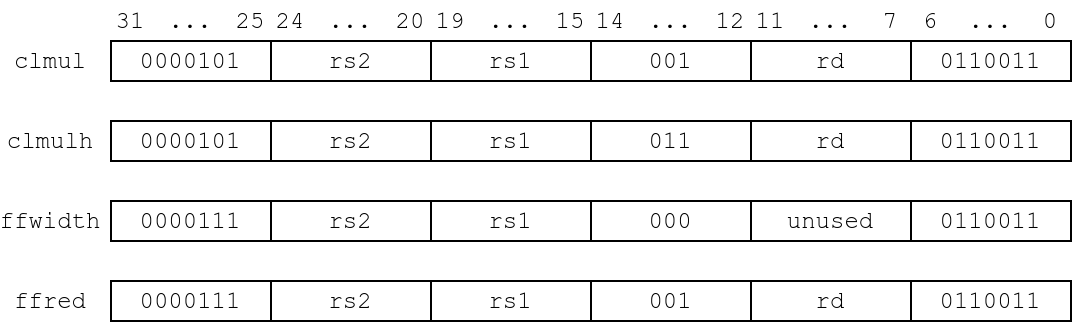
\includegraphics[width=0.8\linewidth]{img/instr.png}
    \caption{The instruction format for the custom Galois field arithmetic instructions.}
    \Description{The instruction format for the custom Galois field arithmetic instructions.}
    \label{fig:instr}
\end{figure*}

\begin{itemize}
    \item \textcolor{blue}{Non-binary error-correction codes (i.e., Non-binary LDPC, BCH, RS codes, \dots)}
    \item \textcolor{blue}{Pre-quantum cryptography (i.e., AES, Elliptic Curve, \dots)}
    \item \textcolor{blue}{PQC cryptography (i.e., McEliece, Rainbow, HQC, \dots)}
\end{itemize}




\section{Proposed ISA extension}
\begin{figure*}[tp]
    \centering
    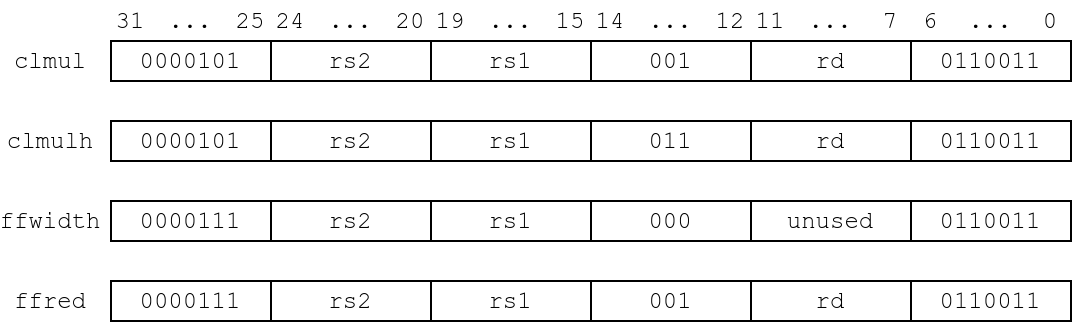
\includegraphics[width=0.8\linewidth]{img/instr.png}
    \caption{The instruction format for the custom galois field arithmetic instructions.}
    \Description{The instruction format for the custom galois field arithmetic instructions.}
    \label{fig:instr}
\end{figure*}

This section describes the ISA extension for RISC-V processors proposed in this work. The selection criteria
of the opcodes were based on the SweRV-EL2 \cite{marena2019risc} microarchitecture. 

The operation added in this extension is the multiplication of finite fields since the sum of two numbers in 
$GF(2^m)$ is only an XOR operation, and it is already defined in RV32I / RV64I. The multiplication is done in three different 
instructions (See Section \ref{section:gf_mult}): carry-less multiplication (CLMULH and CLMUL) and polynomial reduction (FFRED).

To correctly multiply two numbers in $GF(2^m)$, it is also necessary to indicate the irreducible polynomial and the polynomial 
degree to the processor. Therefore, additional instruction is required to pass these parameters (FFWIDTH).

In some processors, such as SweRV-EL2, carry-less multiplication is already implemented in the processor as an extension. Hence, 
the opcode is kept for a compatibility and resource sharing issue.

We decided not to implement the square function and the inverse of $GF(2^m)$ since they are modules that require much logic 
and can also be calculated using finite field multiplication. In more specific computers, these two instructions can be added to 
improve the system's efficiency at the expense of increasing logic utilization.

Figure \ref{fig:instr} shows the formats of the custom instructions proposed in this work. As we can see here, the carry-less multiplication 
keeps the RISC-V extension B format. 

The parameters that receive and return the instructions are:

\begin{itemize}
    \item \textbf{FFWIDTH}: It receives in RS1 the degree of the polynomials, and in RS2, the irreducible polynomial. Since RISC-V registers are 32-bits, 
    the most significant bit of the irreducible polynomial is assumed to be logical 1 when the degree of the input polynomials is 32. For example, for AES, 
    the polynomial degree (RS1) is 8, and the irreducible polynomial (RS2) is 0x11B.
    \item \textbf{FFRED}: It receives the polynomial to be reduced as parameters. In RS1, it receives the high part, and in RS2, the low part of the polynomial. 
    This instruction returns the reduced polynomial $c(x)$. 
    \item \textbf{CLMULH \& CLMUL}: The parameters are the same as extension B.
\end{itemize}

\begin{lstlisting}[caption={GF multiplication for AES},captionpos=b,label={lst:aes}]
li	    a5, 8       % Polynomial degree
li	    a4,283      % Irreducible polynomial
ffwidth	a5,a5,a4    % Load the parameters
...
lbu	    a4,0(a0)
lbu	    a7,0(a1)
clmul	a4,a4,a7    % CL multiplication
li	    a5,0
ffred	a7,a5,a4    % Polynomial reduction
\end{lstlisting}

An example of the multiplication of finite fields using the custom instructions is shown in Listing \ref{lst:aes}. 
This example is a part of the AES code. The FFWIDTH instruction appears only for the first time to tell the hardware 
the polynomial degree and the irreducible polynomial. 
The register RS1 passed to FFRED is 0 because AES uses polynomials that belong to $GF(2^8)$ 
and the bits 63-32 will always be zero after carry-less multiplication.



\section{Implementation results}
\begin{figure}[b]
    \centering
    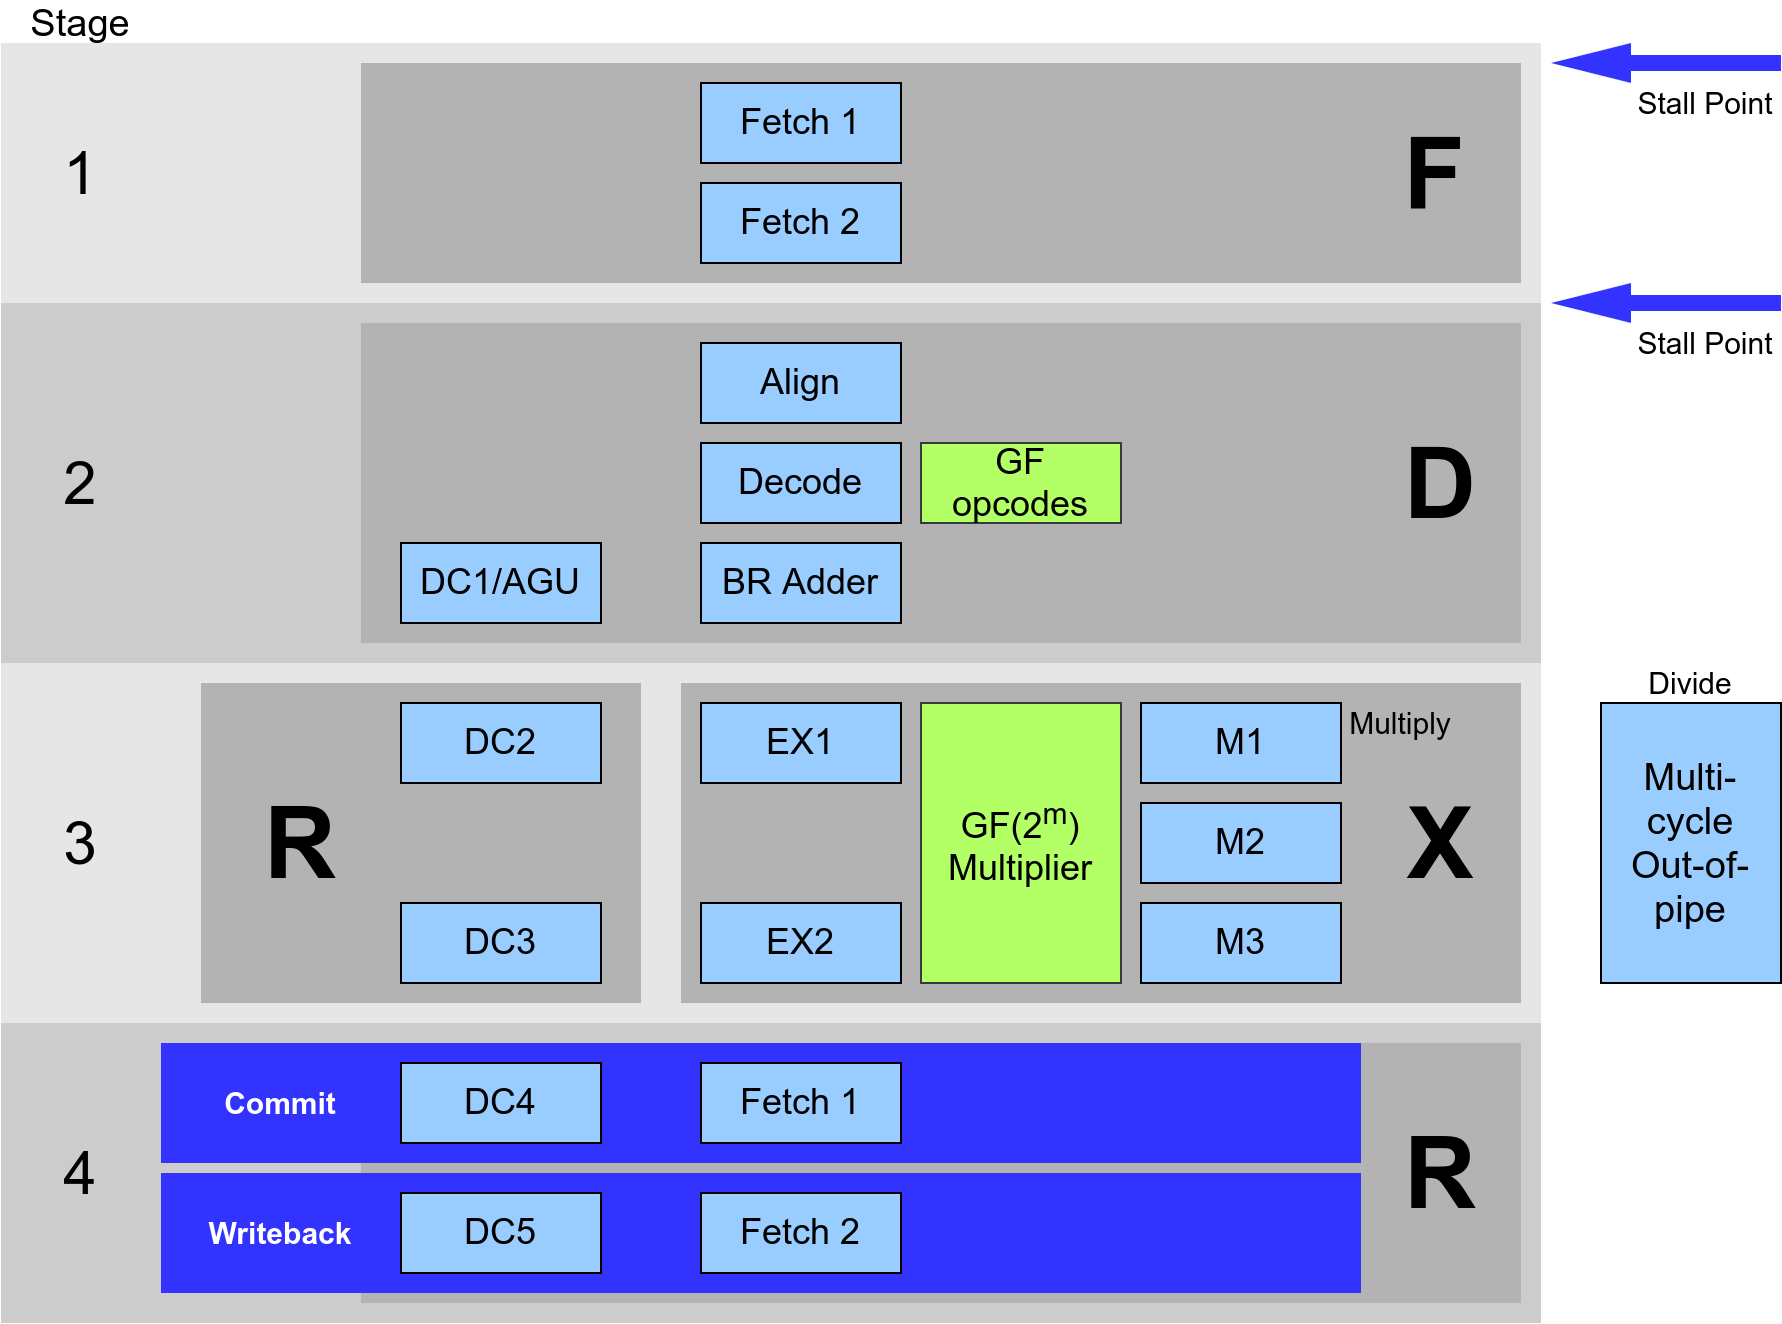
\includegraphics[width=0.95\linewidth]{img/swerv.png}
    \caption{SweRV EL2 Core Pipeline \cite{swervel2}.}
    \Description{SweRV EL2 Core Pipeline.}
    \label{fig:swerv}
\end{figure}

The custom instructions are implemented and validated with Verilator v4.032 using the SweRV-EL2 v1.3 core.

The first step is adding the logic in the decoding stage to recognize the opcode of the custom instructions. 
Espresso logic minimizer \cite{250190} is used in this stage.

Then, the corresponding logic is added in the execution stage. Since carry-less multiplication and binary 
multiplication share the same module within the core, the polynomial reduction module is also implemented 
in the same block. The block diagram of the SweRV-EL2 core is shown in Fig. \ref{fig:swerv}.

Once the logic is implemented, the assembly module (binutils) is modified. Thus, the toolchain can recognize 
the opcodes of the custom instructions. Binutils is a collection of 
binary tools and part of the RISC-V GNU toolchain, including the assembler and the linker.
In this way, we can run tests of different algorithms using the C language and compare the efficiency between the RV32IMC base and custom instructions. 
In this work, a performance evaluation for AES and Reed-Solomon codes is made.

\subsection{AES performance} 

The C code was generated for the different key sizes (AES128, AES192, and AES256) and encryption schemes (CBC, CTR, and ECB). Another version was created with the custom instructions replacing
the code segments where the GF multiplication appears. 
Then, they were compiled with the following flags: 

\begin{center}
\textbf{-O3 -fomit-frame-pointer -fPIC -no-pie}
\end{center}

\begin{table}[b]
    \begin{tabular}{ccclcc}
    \multicolumn{1}{l}{}              & \multicolumn{2}{c}{\cellcolor[HTML]{C0C0C0}RS(255,247)}         &                          & \multicolumn{2}{c}{\cellcolor[HTML]{C0C0C0}RS(255,239)}         \\
    \cellcolor[HTML]{FFFFFF}          & \cellcolor[HTML]{C0C0C0}Encode & \cellcolor[HTML]{C0C0C0}Decode & \cellcolor[HTML]{FFFFFF} & \cellcolor[HTML]{C0C0C0}Encode & \cellcolor[HTML]{C0C0C0}Decode \\ \hline
    \cellcolor[HTML]{EFEFEF}standard   & 154,003                         & 151,681                         &                          & 300,831                         & 303,289                         \\
    \cellcolor[HTML]{EFEFEF}out proposal    & 29,006                          & 22,648                          &                          & 58,660                          & 45,237                          \\
    \cellcolor[HTML]{EFEFEF}Reduc. \% & 81.17\%                          & 85.07\%                          &                          & 80.50\%                          & 85.08\%                         
    \end{tabular}
    \caption{Number of clock cycles required for RS codes.}
    \label{tab:rs}
\end{table}

\begin{table*}[tp]
    \begin{tabular}{ccccccc}
    \rowcolor[HTML]{C0C0C0} 
    AES128                               & CBC Enc.             & CBC Dec.             & CTR Enc.             & CTR Dec.             & ECB Enc.             & ECB Dec.             \\ \hline
    \cellcolor[HTML]{EFEFEF}standard     & 197,920              & 198,240              & 198,208              & 198,197              & 50,641               & 50,726               \\
    \cellcolor[HTML]{EFEFEF}our proposal & 38,328               & 39,303               & 39,033               & 38,995               & 10,854               & 11,011               \\
    \cellcolor[HTML]{EFEFEF}Reduc. \%    & 80.63\%                & 80.17\%                & 80.31\%                & 80.33\%                & 78.57\%                & 78.29\%                \\
    \multicolumn{1}{l}{}                 & \multicolumn{1}{l}{} & \multicolumn{1}{l}{} & \multicolumn{1}{l}{} & \multicolumn{1}{l}{} & \multicolumn{1}{l}{} & \multicolumn{1}{l}{} \\
    \rowcolor[HTML]{C0C0C0}AES192       & CBC Enc.             & CBC Dec.             & CTR Enc.             & CTR Dec.             & ECB Enc.             & ECB Dec.             \\ \hline
    \cellcolor[HTML]{EFEFEF}standard     & 242,573              & 242,695              & 242,839              & 242,828              & 62,572               & 62,661               \\
    \cellcolor[HTML]{EFEFEF}our proposal & 47,016               & 48,019               & 47,637               & 47,617               & 13,764               & 13,939               \\
    \cellcolor[HTML]{EFEFEF}Reduc. \%    & 80.62\%                & 80.21\%                & 80.38\%                & 80.39\%                & 78.00\%                & 77.75\%                \\
    \multicolumn{1}{l}{}                 & \multicolumn{1}{l}{} & \multicolumn{1}{l}{} & \multicolumn{1}{l}{} & \multicolumn{1}{l}{} & \multicolumn{1}{l}{} & \multicolumn{1}{l}{} \\
    \rowcolor[HTML]{C0C0C0}AES256       & CBC Enc.             & CBC Dec.             & CTR Enc.             & CTR Dec.             & ECB Enc.             & ECB Dec.             \\ \hline
    \cellcolor[HTML]{EFEFEF}standard     & 285,245              & 285,593              & 285,439              & 285,425              & 72,331               & 72,416               \\
    \cellcolor[HTML]{EFEFEF}our proposal & 53,396               & 54,548               & 54,054               & 54,036               & 14,462               & 14,660               \\
    \cellcolor[HTML]{EFEFEF}Reduc. \%    & 81.28\%                & 80.90\%                & 81.06\%                & 81.07\%                & 80.01\%                & 79.76\%               
    \end{tabular}
    \caption{Number of clock cycles required for AES (RV32IMC vs custom).}
    \label{tab:aes}
\end{table*}
\begin{table*}[tp]
    \begin{tabular}{ccccccc}
    %\rowcolor[HTML]{C0C0C0} 
    %SweRVolf                        & Slice LUTs           & Slice Registers      & F7 Muxes             & F8 Muxes             & Slice                          & LUT as logic         & LUT as memory        & Block RAM            \\ \hline
    %\cellcolor[HTML]{EFEFEF}std     & 24714                & 12969                & 459                  & 78                   & \cellcolor[HTML]{FFCE93}7115   & 24427                & 287                  & 14                   \\
    %\cellcolor[HTML]{EFEFEF}custom  & 26073                & 13006                & 531                  & 84                   & \cellcolor[HTML]{FFCE93}7521   & 25786                & 287                  & 14                   \\ \hline
    %\cellcolor[HTML]{EFEFEF}Inc. \% &                      &                      &                      &                      & \cellcolor[HTML]{FFCE93}5.71\% &                      &                      &                      \\
    %\multicolumn{1}{l}{}            & \multicolumn{1}{l}{} & \multicolumn{1}{l}{} & \multicolumn{1}{l}{} & \multicolumn{1}{l}{} & \multicolumn{1}{l}{}           & \multicolumn{1}{l}{} & \multicolumn{1}{l}{} & \multicolumn{1}{l}{} \\
    \rowcolor[HTML]{C0C0C0} 
    SweRV-EL2                       & Slice LUTs           & Slice Registers      & F7 Muxes             & F8 Muxes             & Slice                          & LUT as logic                   \\ \hline
    \cellcolor[HTML]{EFEFEF}standard     & 18,605                & 7651                 & 341                  & 74                   & 5,329   & 18,605                                   \\
    \cellcolor[HTML]{EFEFEF}our proposal  & 19,974                & 7688                 & 413                  & 80                   & 5,699   & 19,974                                   \\ \hline
    \cellcolor[HTML]{EFEFEF}Inc. \% & 7.36\%                     &    0.48\%                  & 21.11\%                     &  8.11\%                    & 6.94\% & 7.36\%                                           
    \end{tabular}
    \caption{Logic utilization of SweRV-EL2 core, implemented on a Nexys A7 FPGA.}
    \label{tab:area}
\end{table*}

The \textbf{typical\_pd} and \textbf{fpga\_optimize} settings were used for the SweRV-EL2 core. These configurations create a lightweight processor to implement on the Nexys A7 FPGA.

Table \ref{tab:aes} shows the number of clock cycles required for the base and custom instructions for each encryption method. It can be seen that for all of the cases, a significant reduction of 77.75\% can be reached. 
For example, for AES256, the clock cycles needed for CBC encryption is 285,245, while using our proposal only needs 53,396.

Regarding the code size reduction, it was observed that it is greater than 35\% for all cases.

\subsection{Reed-Solomon performance} 

The same was done for the Reed-Solomon code performance comparison. A program in C code has been created with the encryption and decryption routine for RS(255,247) and RS(255,239). And then, another 
version was created with the custom instructions, replacing the multiplication of finite fields.

The same SweRV-EL2 configurations as for AES were kept, and they were also compiled with the same GCC flags.

Table \ref{tab:rs} shows the number of clock cycles required to encrypt and decrypt the RS(255,247) and RS(255,239) codes. 
As we can see here, for example, the clock cycles required to encode in RS(255,247) have been reduced by 81.17\%, 
being 154,003 for RV32IMC and 29,006 for our proposal.

\subsection{Logic utilization} 

In order to implement in an FPGA (Nexys A7), the SweRV-EL2 core was integrated into SweRVolf \cite{swervolf} SoC, 
which consists of the SweRV CPU with a boot ROM, AXI4 interconnect, UART, SPI, \mbox{RISC-V} timer, and GPIO. %(See Fig. \ref{fig:swervolf}).

Two different SoC versions were created, one with the base instructions and the other with the custom instructions, 
both with the extension Zbc \cite{swervel2} enabled.

Table \ref{tab:area} shows the logic utilization for the standard and custom version. It can be seen that there is a 6.94\% increase in the 
number of slices.

Regarding the clock frequency, both work at 50 MHz. There was no decrease in frequency due to the addition of the extra logic for the
custom instructions.

%\begin{figure}[t]
%    \centering
%    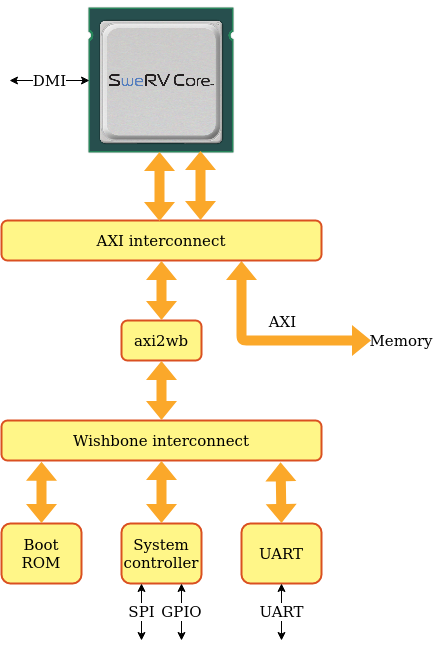
\includegraphics[width=0.7\linewidth]{img/swervolf.png}
%    \caption{SweRVolf \cite{swervolf} core block diagram.}
%    \Description{SweRVolf \cite{swervolf} core block diagram.}
%    \label{fig:swervolf}
%\end{figure}



\section{Conclusions}
Due to the rise of Edge Computing \cite{7488250}, small portable devices have to process 
efficiently different error correction codes, cryptography, 
and in some cases, proprietary protocols.

Finite field $GF(2^m)$ arithmetic has been identified to be used in many applications, such as pre-quantum cryptography, and error correction codes. Therefore, an extension of the instructions is proposed in this work. 
It is oriented to applications where it is necessary to process different protocols that use finite field arithmetic.

From the previous section, it can be seen that for AES and Reed-Solomon, a reduction of 77.75\% was achieved 
in the number of clock cycles at the expense of a 6.94\% increment in logic utilization.

\textcolor{blue}{As future work, we are using these instructions for post-quantum cryptography. The Classic McEliece and HQC algorithms are adapted to the RISC-V architecture. We are in the stage of evaluating its performance and extracting results.}


%\section{Acknowledgments}

%Identification of funding sources and other support, and thanks to
%individuals and groups that assisted in the research and the
%preparation of the work should be included in an acknowledgment
%section, which is placed just before the reference section in your
%document.

%%
%% The next two lines define the bibliography style to be used, and
%% the bibliography file.
\bibliographystyle{ACM-Reference-Format}
\bibliography{sample-base}



\end{document}
\endinput
%%
%% End of file `sample-sigconf.tex'.
